\documentclass[reqno,twoside]{amsart}
\usepackage{amsmath}
\usepackage{amssymb}
\usepackage[colorlinks=true, pdfstartview=FitV, linkcolor=blue, citecolor=blue, urlcolor=blue]{hyperref}
\usepackage{color}
\usepackage{tikz}
\usetikzlibrary{decorations.markings, decorations.pathmorphing, arrows.meta}
\tikzset{
    >=Stealth,
    branch cut/.style={decorate, decoration={snake, amplitude=1pt, segment length=3pt}},
    mid arrow/.style={postaction={decorate, decoration={markings, mark=at position #1 with {\arrow{>}}}}},
    mid arrow/.default=0.5
}
\usepackage[breakable, theorems, skins]{tcolorbox}
\usepackage{tikz}
\usetikzlibrary{arrows.meta}
\usetikzlibrary{decorations.markings}
\tikzset{->-/.style={decoration={
  markings,
  mark=at position #1 with {\arrow{>}}},postaction={decorate}}}
\tikzset{middlearrow/.style={
        decoration={markings,
            mark= at position 0.55 with {\arrow{#1}} ,
        },
        postaction={decorate}
    }
}

\begin{document}

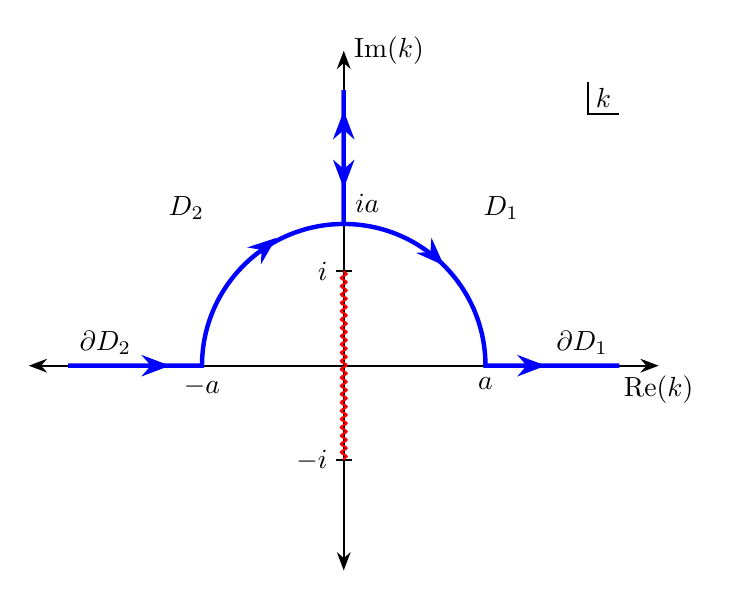
\begin{tikzpicture}[>=Stealth]

    \draw[<->,thick] (-4,0) -- (4,0) node[below]{Re($k$)};
    \draw[<->,thick] (0,-2.6) -- (0,4.0) node[right]{Im($k$)};

    \draw[thick] (-0.1, 1.2) -- (0.1, 1.2) node[left=5pt] {$i$}; 
     \draw[thick] (-0.1, -1.2) -- (0.1, -1.2) node[left=5pt] {$-i$}; 

      \draw[red, thick, branch cut] (0,1.2) -- (0,-1.2);


    \draw[blue, ultra thick, 
        decoration={markings, 
            mark=at position 0.2 with {\arrow{>}}, 
            mark=at position 0.5 with {\arrow{>}}, 
            mark=at position 0.85 with {\arrow{>}}}, 
        postaction={decorate}]
        (0.0, 3.5) -- (0.0, 1.8) node[above right]{\color{black}{$ia$}}
        arc[start angle=90, end angle=0, radius=1.8] node[below]{\color{black}{$a$}}
        -- (3.5, 0.0)
        node[above left, black] {$\partial D_1$};
        %
         \draw[blue, ultra thick, 
        decoration={markings, 
            mark=at position 0.1 with {\arrow{<}}, 
            mark=at position 0.47 with {\arrow{<}}, 
            mark=at position 0.85 with {\arrow{<}}}, 
        postaction={decorate}]
        (0.0, 3.5) -- (0.0, 1.8)
        arc[start angle=90, end angle=180, radius=1.8] 
        node[below]{\color{black}{$-a$}}
        -- (-3.5, 0.0)
        node[above right, black] {$\partial D_2$};

  \node at (2, 2) {$D_1$};
  \node at (-2, 2) {$D_2$};
  
\begin{scope}[shift={(3.1,3.2)}]
        \draw[thick] (0,0.4) -- (0,0) -- (0.4,0);
        \node at (0.2, 0.2) {$k$};
    \end{scope}

\end{tikzpicture}

\end{document}